\chapter{Introducción específica} % Main chapter title

\label{Chapter2}

%----------------------------------------------------------------------------------------
%	SECTION 1
%----------------------------------------------------------------------------------------
%
%En este capítulo deberías tener:
%1. Conversores AD.  Describir con detalles técnico lo básico de la tecnología que usaste, con lo necesario para que se comprenda lo que sigue en el cap 3.  Usar citas bibliográficas.  Explicar el proceso de cuantización, codificación, el error en la conversión, bits de resolución, ruido, etc.
%Acá podría ir cualquier otro aspecto tecnológico/herramientas que hayas utilizado y quieras documentar, por ejemplo protocolos de comunicación o aspectos metodológicos que hayas seguido como TDD o uso de repositorios de software, etc.
%2. Planificación. Aspectos relevantes de la planificación que ayuden a entender cómo se hizo el trabajo.  El AoN suele ser adecuado para eso.  Algo que te sirva para retomarlo en las conclusiones (riesgos,supuestos,gantt,etc)
%3. Requerimientos
%
%Explicar los detalles que el lector debe conocer para entender las decisiones de diseño adoptadas.

% A continuación se describirán diferentes tecnologías usadas en el trabajo que hicieron posible al trabajo desarrollado.

En el presente capítulo se describe el microcontrolador que se eligió para el trabajo, los métodos de medición usados y las herramientas de software desarrolladas por terceros que se utilizaron.

\section{Microcontrolador principal}
\label{sec:cap2parte1}

%En este sistema embebido el microcontrolador ocupa un rol principal pues las demás estructuras que se diseñan dependen de este para funcionar, o mejor dicho se diseñan para ser controladas por este. 

El trabajo realizado implicó el desarrollo de un producto electrónico que debe efectuar diferentes tareas, como medir, comunicar y en algunos casos accionar. Uno de los elementos que hace posible el funcionamiento del sistema es el microcontrolador, que es el encargado de realizar las diferentes tareas que el dispositivo debe llevar a cabo. 

Para este trabajo se optó por un microcontrolador que pueda ser usado para una aplicación de medición y que sea de bajo consumo eléctrico. 

%Como toda aplicación de un sistema embebido, la electrónica diseñada suele ser mas una extension del microcontrolador, adaptado analógicamente para que realice las tareas que se desea resolver, que una parte más de la electrónica.

El microcontrolador elegido para el dispositivo fue un MSP430F2618 \cite{msp430freff}, fabricado por la empresa Texas Instruments. Este microcontrolador es de ultra baja potencia y posee una CPU de instrucciones RISC de 16 bits. Este microcontrolador, cuyo \textit{pinout} se puede observar en la figura \ref{fig:msp430squematic}, puede pasar de sus distintos modos de baja potencia al modo activo en menos de un 1 $\mu$s.


%\begin{figure}[!h]
%	\centering
%	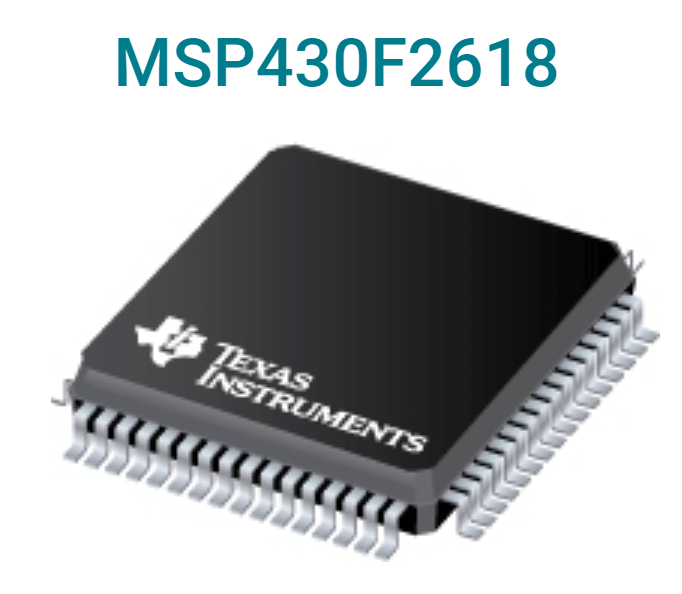
\includegraphics[width=40mm,keepaspectratio]{Figures/msp430F2618.png}
%	\caption{Ilustración del micro controlador como se lo presenta en la pagina web %del fabricante.}
%	\label{fig:msp430imagen}
%\end{figure}

El MSP430F2618 posee en su estructura interna diferentes tipos de periféricos ideados para diversas aplicaciones. El fabricante denomina a cada uno de estos periféricos como \textquotedblleft módulos\textquotedblright .
 
Estos módulos son hardware de diferentes aplicaciones que normalmente usan los microcontroladores, los cuales el fabricante decidido incluirlos en el circuito integrado. El MSP430F2618 incluye por ejemplo un módulo de reloj, un módulo controlador de memoria flash, un módulo de comunicación serie y un módulo de control directo de memoria (DMA) \cite{msp430slau144j}. 

Como los módulos se encuentran en el circuito integrado, estos están conectados a la CPU a través de buses de dato, dirección y control. Los módulos se pueden utilizar  accediendo a las direcciones de memoria correspondientes. El uso de estos módulos facilita la programación del firmware, y añade al microcontrolador diferentes capacidades sin agregar hardware extra.


Este modelo de la familia MSP430 \citep{msp430family} se eligió específicamente por poseer tanto un módulo ADC (conversor analógico-digital) cómo un módulo DAC (conversor digital-analógico). El módulo DAC fue utilizado para la implementación de un lazo de corriente \citep{liptak2018instrument}, que es una forma de comunicación común para procesos industriales. Se consideró usar al módulo ADC para realizar mediciones de corriente o tensión, sin embargo su uso fue descartado por otra solución más completa que involucraba a otro circuito integrado.

Para el trabajo se usó el módulo de comunicación serie universal(UART) del MSP430 para realizar la comunicación con el integrado de medición como también para realizar los protocolos de comunicación requeridos. Para asegurar la estabilidad de las comunicaciones seriales como también para aumentar la precisión de los módulos temporizadores dentro del microcontrolador se decidió implementar un oscilador externo.

\begin{figure}[!h]
	\centering
	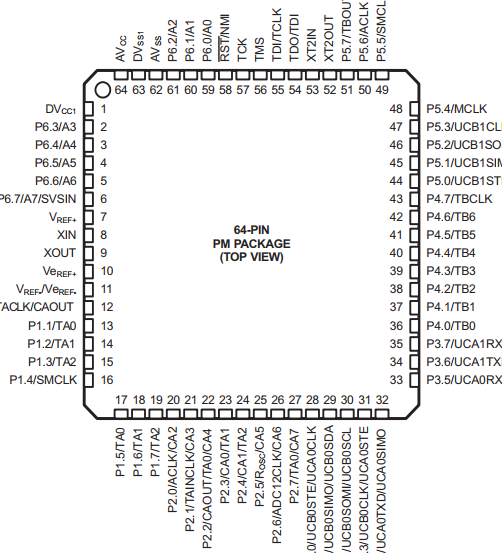
\includegraphics[width=60mm,keepaspectratio]{Figures/microdatasheet1.png}
	\caption{Esquemático del \textit{pinout} de un microcontrolador MSP430F261x.}
	\label{fig:msp430squematic}
\end{figure}

%\renewcommand{\mkcitation}[1]{ (#1)}
%\renewcommand{\mktextquote}[6]{#1#2#3#6#4#5}

%En cuanto al empaquetado del dispositivo se optó por el de 64 pines de salida (denominado por el fabricante como \textquotedblleft LQFP-64 Texas Instruments\textquotedblright ) que puede verse en la figura \ref{fig:paquet64}. Esta versión a diferencia del empaquetado de 80 pines posee más de una implementación de módulos por pin. Debido a que no se iban a usar todas las prestaciones del microcontrolador esto no presentaba un problema. 

%\begin{figure}[!h]
%	\centering
%	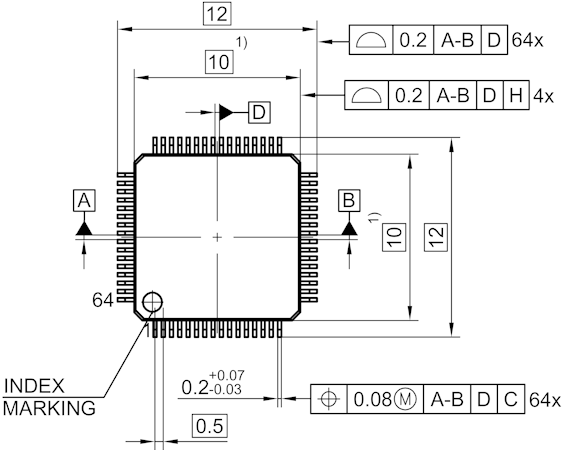
\includegraphics[width=80mm,keepaspectratio]{Figures/PG-LQFP-64-18.png}
%	\caption{Dimensiones del empaquetado LQFP-64 (valores en milímetros).}
%	\label{fig:paquet64}
%\end{figure}

%El empaquetado de montaje superficial es de un tamaño bastante pequeño (sus dimensiones son de 12x12 mm) por lo que presentaba un pequeño desafío al implementarlo en el diseño del PCB.


\section{Herramientas de programación}
\label{sec:cap2parte2}
\subsection{FET \textit{debugger}}

%Para lograr que el microcontrolador realice todas las tareas requeridas se debe programarlo para tal fin, es decir se debe escribir las instrucciones que deberá seguir el microcontrolador. El conjunto de instrucciones que se escriben para que un microcontrolador funcione es a lo que denominamos programa, y en este trabajo se llamara firmware. El firmware debe cargarse de algún modo desde la computadora personal donde lo diseñamos al chip. 

Para cargar el programa al microcontrolador, el fabricante especifica una herramienta de programación al que denomina \textquotedblleft FET hardware JTAG\textquotedblright \cite{FETjtag} , donde FET es acrónimo de \textit{Flash Emulation Tool} y JTAG acrónimo de \textit{Joint Test Action Group}. La herramienta puede verse en la figura \ref{fig:mspFETtool}. El JTAG es un estándar industrial para verificar diseños y testear placas de circuito impresas después de manufacturadas \cite{JTAGintel}. 
%Los programadores JTAG son usados para escribir software en memorias \textit{flash}.
%citar el resumen de intel del ieee

%JTAG (named after the Joint Test Action Group which codified it) is an industry standard for verifying designs and testing printed circuit boards after manufacture.
%Although JTAG's early applications targeted board level testing, here the JTAG standard was designed to assist with device, board, and system testing, diagnosis, and fault isolation. Today JTAG is used as the primary means of accessing sub-blocks of integrated circuits, making it an essential mechanism for debugging embedded systems which 

\begin{figure}[!h]
	\centering
	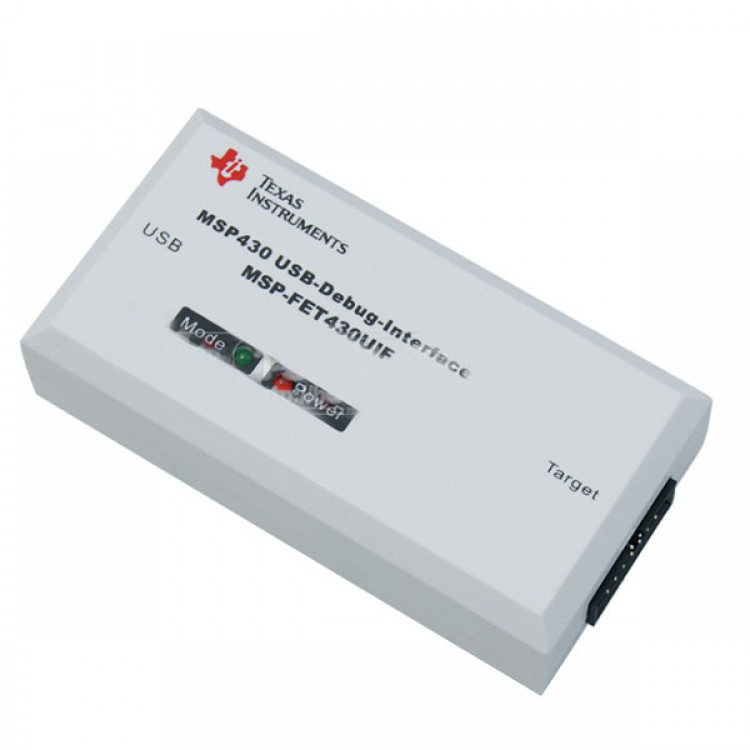
\includegraphics[width=100mm,keepaspectratio]{Figures/emeesepeFET.jpg}
	\caption{ Foto del MSP-FET430UIF, que es la herramienta de programación del microcontrolador.}
	\label{fig:mspFETtool}
\end{figure}

Con las conexiones apropiadas, un debugger y la interfaz JTAG pueden ser usadas para depurar código en el microcontrolador. Esto facilita la programación de prototipos a realizar. 


%The typical MSP Flasher execution flow consists of the following steps. Optional steps can be activated or
%deactivated by using special triggers or parameters (see Section 3).
%1. Initialize FET debugger
%2. Perform FET recovery (if a corrupted FET firmware is detected)
%3. Update FET firmware (if a mismatch between firmware and MSP Debug Stack versions is detected)
%4. Power up the target MSP device
%5. Configure the target MSP for JTAG or SBW communication
%6. Connect to the target MSP and display device information
%7. Optional: Erase (parts of) the target device memory
%8. Optional: Load target code into the device from a TXT or HEX file
%9. Optional: Verify target code transfer
%10. Optional: Read device memory and write it to a TXT or HEX file
%11. Optional: Reset the device
%12. Optional: Lock JTAG access
%13. Optional: Reset the device
%14. Optional: Power down the device
%15. Optional: Start target code execution
%16. Disconnect from the target MSP device
%17. Close the FET connection

%citar datasheet del msp

%\begin{figure}[!h]
%	\centering
%	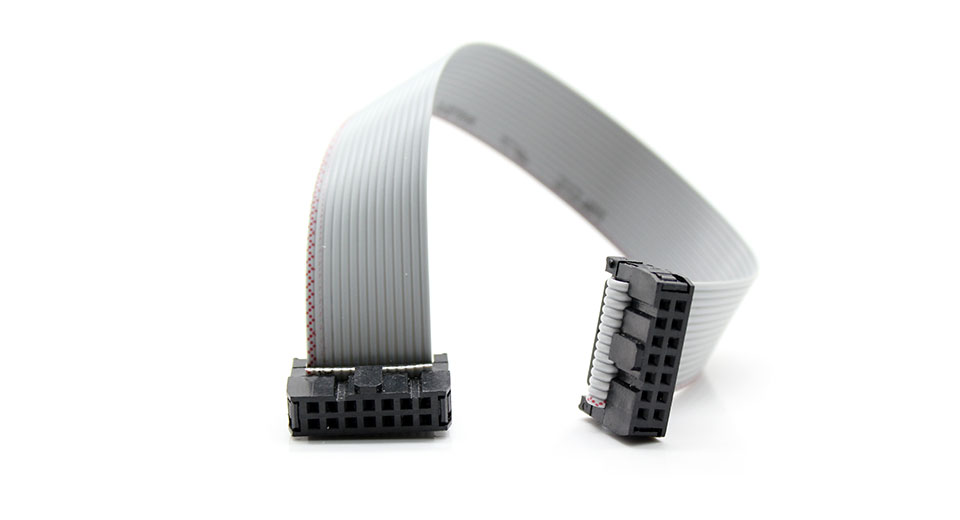
\includegraphics[width=120mm,keepaspectratio]{Figures/cableJtag.jpg}
%	\caption{ Cable conector de la interfaz JTAG. }
%	\label{fig:mspFETcable}
%\end{figure}

En la hoja de datos de la herramienta, el fabricante especifica las conexiones y funciones de cada pin, como puede verse en la figura \ref{fig:JtagSCH}.


El circuito esquemático de las conexiones fue tomado en cuenta para el diseño del esquemático del prototipo, en el cual se optó por una interfaz \textit{JTAG Through-Hole}, ya que era la conexión requerida de la herramienta de programación disponible. 
% \textit{pin header}

Para el trabajo realizado, la empresa SERVAIND S.A. proveyó la herramienta MSP-FET430UIF \cite{FETjtag} para poder entender y probar el proceso de programación de un microcontrolador MSP430.


\begin{figure}[!h]
	\centering
	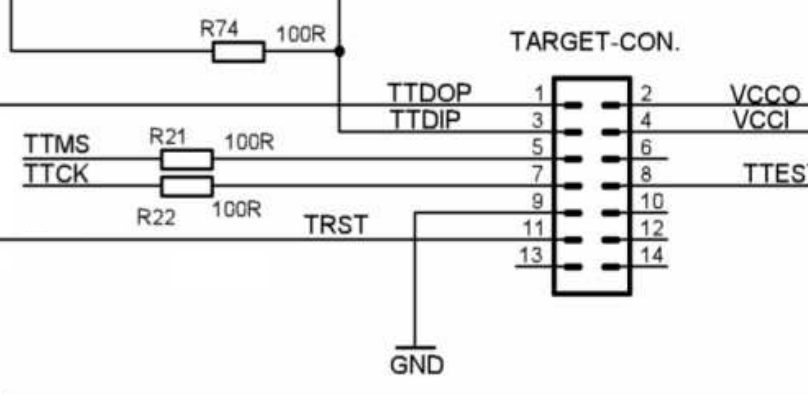
\includegraphics[width=100mm,keepaspectratio]{Figures/Jtagfetsch.png}
	\caption{ Esquemático del conector JTAG de la herramienta de programación. }
	\label{fig:JtagSCH}
\end{figure}

%The MSP debug stack (MSPDS) for all MSP430™ microcontrollers (MCUs) and SimpleLink™ MSP432™ devices consists of a static library on the host system side as well as an embedded firmware that runs on debug tools including the MSP-FET, MSP-FET430UIF or on-board eZ debuggers. It is the bridging element between all PC software and all MSP430 and SimpleLink MSP432 microcontroller derivatives and handles tasks such as code download, stepping through code or break points. The MSP Debug Stack is used in integrated development environments such as Code Composer Studio™ (CCS), IAR's Embedded Workbench or tools like Smart RF Studio and Elprotronic's FlashPro430.


\subsection{Entorno de desarrollo}
\subsubsection{ El MSP Debug Stack}

Para poder programar el microcontrolador, el fabricante ofrece una solución de software denominada \textquotedblleft MSPDS\textquotedblright \ que significa \textit{MSP Debug stack}. El \textit{MSP Debug stack} es una biblioteca dinámica que provee funciones para controlar y depurar microcontroladores de la familia MSP40 durante la fase de desarrollo de software. El \textit{MSP Debug stack} controla al MSP430 a través de la interfaz JTAG. La biblioteca provee control de dispositivo, programación de memoria y funcionalidad de depuración, por ejemplo \textit{breakpoints} \cite{GuideMSPStack}.

Esta biblioteca simplifica el controlar el MSP430 aislando al usuario de las complejidades del protocolo JTAG. Además, la biblioteca puede conectarse a un MSP430 objetivo sin parar o cambiar la ejecución del programa.

%El MSPDebugStack
El \textquotedblleft stack debug de MSP\textquotedblright \ es diseñado para los microcontroladores de la familia MSP430. Consiste en una biblioteca estática en el lado del host (donde se realizan los programas) y de un firmware embebido que corre herramientas de depuración para el MSP-FET \cite{GuideMSPStack}.

\subsubsection{Entorno de desarrollo}

%If you intend to program your MSP430 or MSP432 device out of an IDE, simply download the latest version of Code Composer Studio or IAR Embedded Workbench release. The latest MSP Debug Stack will be inclu

Para realizar el programa en lenguaje C, el fabricante del microcontrolador recomienda al IDE (Entorno de Desarrollo Integrado) \textquotedblleft IAR Embedded Workbench\textquotedblright , ya que este software incluye al  MSP Debug Stack, por lo que no hay que escribir archivos \textit{ make file} o hacer una compilación manual ya que esto lo soluciona el entorno.

Para el trabajo realizado la empresa SERVAIND S.A. proveyó una versión del IDE IAR, con el fin de acelerar el proceso de desarrollo del software. Una ventana del entorno de desarrollo puede verse en la figura \ref{fig:IARwindow}.

\begin{figure}[h]
	\centering
	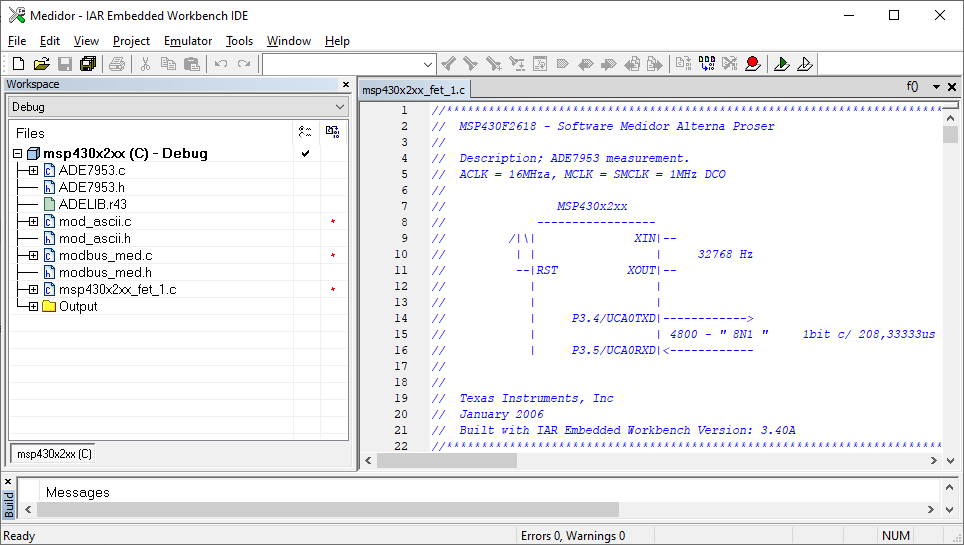
\includegraphics[width=\textwidth,keepaspectratio]{Figures/Embeddedworkbench.png}
	\caption{Imagen del entorno de desarrollo.}
	\label{fig:IARwindow}
\end{figure}

%citar datashet del fet


\section{Circuito integrado de medición}
\label{sec:cap2parte3}

Para la realización de este trabajo se decidió utilizar un chip que soluciona las complejidades de los cálculos de medición de una red eléctrica, el integrado de medición seleccionado fue el denominado ADE7953, cuyo fabricante es Analog Devices. El ADE7953 es un SOC (\textit{System On Chip}) de medición de energía eléctrica de alta precisión, con el propósito de aplicaciones monofásicas. Mide tensión y corriente de línea y calcula energía activa, reactiva y aparente. El dispositivo incorpora tres ADC sigma-delta con un núcleo de medición de energía de alta precisión. 

La estructura del ADE7953 adapta un AFE (analog front end) a una interfaz digital, de manera que los valores que mide el circuito integrado sean fácilmente accesibles en forma de registros de datos, los cuales se pueden acceder por protocolos de comunicación comunes como UART, I2C o SPI.
%citar datasheet ADE7953

%Explicar que es lo que facilita
%%%

Un AFE (\textit{Analog Front End}) es un conjunto de circuitos que acondicionan señales usando amplificadores analógicos sensibles \cite{horlin2008digital}, comúnmente amplificadores operacionales, filtros y circuitos integrados para aplicaciones específicas. De esta manera un AFE provee un bloque electrónico funcional, flexible y configurable, que es necesario para ser interfaz de una variedad de sensores, conversores digitales o microcontroladores.

En el campo de las mediciones eléctricas, los chips AFE son circuitos integrados resultados de una combinación de circuitos analógicos con digitales. Estos suelen ser implementaciones de DAC, tensiones de referencia tipo bandgap, módulos de manejo de potencia, módulos de control, cálculos de medición o conversores de pulsos de energía, por lo que se puede seleccionar un AFE para una aplicación especifica.
%(para sensores, receptores de radio y otros circuitos)
%%citar Vol

%De acuerdo con la \textit{Virtual Socket Interface Aliance}, un \textit{System On Chip} se define como un dispositivo altamente integrado. Es también conocido como un sistema en silicio.

%System on chip puede ser definido como un circuito integrado complejo que consiste en uno o más núcleos programables, conectados usando un bus en chip con núcleo de procesamiento de señales (digitales o analógicas), y que pueden incorporar memoria en chip \cite{badawy2002system}. 

El ADE7953 es un system on chip que posee registros de memoria para facilitar el uso de los datos resultados de las mediciones. Su diagrama funcional puede verse en la figura \ref{fig:ADEfuncbloc}.

\begin{figure}[h]
	\centering
	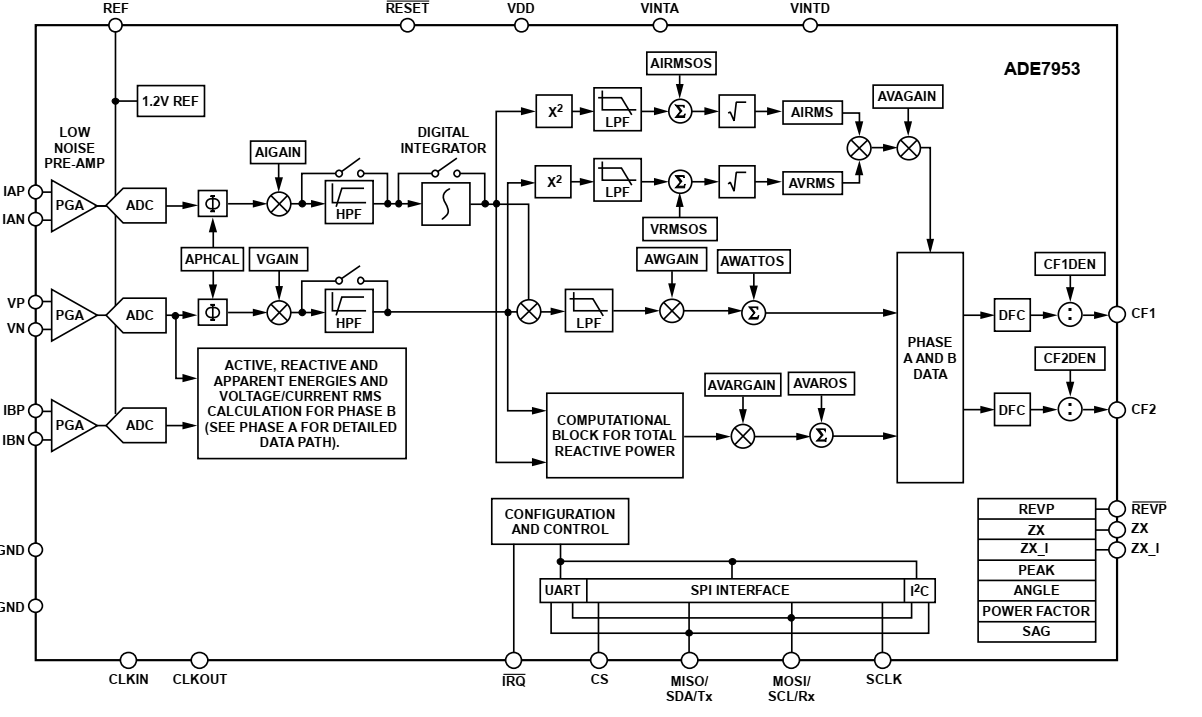
\includegraphics[width=\textwidth , keepaspectratio]{Figures/ade7953funcdiagr.png}
	\caption{Diagrama de bloques funcionales del ADE7953.}
	\label{fig:ADEfuncbloc}
\end{figure}

Del diagrama puede verse los puertos de entrada para la medición, que son IAP, IAN, VP, VN, IBP, IBN, que sirven para realizar una medición monofásica con corriente de neutro, también se observan los diferentes bloques por los cuales la señales se procesan y los registros relacionados, por ejemplo, puede observarse como el registro de ganancia de tensión (VGAIN) y corriente eléctrica (AIGAN) interactúan con la salida del ADC.

El ADE7953 puede comunicarse con un microcontrolador por tres diferentes protocolos: I2C, SPI y UART, para esto deben realizarse las conexiones necesarias. Estos modos de comunicación facilitan la lectura de los datos de los registros. El circuito integrado utiliza diferentes protocolos, según se configure la lógica de los pines. En el modo UART, se puede acceder a todas las funciones del circuito integrado usando solo dos pines de dirección única, donde el ADE7953 actúa como esclavo, toda comunicación se inicia cuando el master envía el frame valido. El formato del frame puede verse en la figura \ref{fig:UARTADE7953}.

\begin{figure}[h]
	\centering
	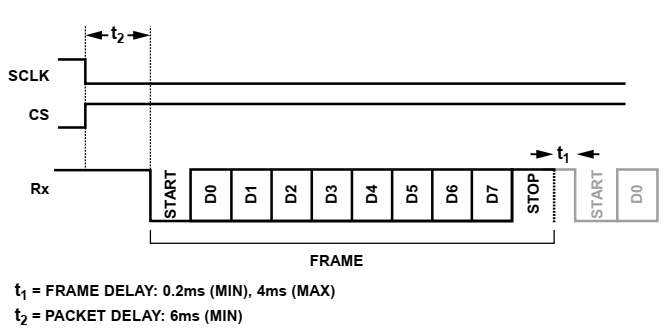
\includegraphics[width=110mm,keepaspectratio]{Figures/tramauartade.png}
	\caption{Trama de protocolo UART del ADE7953.}
	\label{fig:UARTADE7953}
\end{figure}

%JTAG programmers are also used to write software and data into flash memory. This is usually done using the same data bus access the CPU would use, and is sometimes handled by the CPU. In other cases the memory chips themselves have JTAG interfaces. Some modern debug architectures provide internal and external bus master access without needing to halt and take over a CPU. In the worst case, it is usually possible to drive external bus signals using the boundary scan facility.

%This manual describes the hardware of the Texas Instruments MSP-FET430 Flash Emulation Tool (FET).
%The FET is the program development tool for the MSP430 ultra-low-power microcontroller. Both available
%interface types, the parallel port interface and the USB interface, are described.


%If you intend to program your MSP430 or MSP432 device out of an IDE, simply download the latest version of Code Composer Studio or IAR Embedded Workbench release. The latest MSP Debug Stack will be included.



%\subsection{Uso de mayúscula inicial para los título de secciones}

\section{ Biblioteca Externa - Freemodbus}
\label{sec:cap2parte6}

Como el dispositivo a utilizar es pensado para un ambiente industrial, se implementó un protocolo Modbus para la comunicación de este con otros dispositivos, ya que Modbus es sofwtare libre de fácil de implementación.

El protocolo de comunicaciones serial Modbus, es un estándar de facto en la industria, diseñado para integrar PLC, computadoras, terminales, sensores y actuadores. Modbus es un sistema maestro/esclavo, donde un dispositivo, el nodo maestro, controla todas las actividades seriales encuestando selectivamente a los dispositivos esclavos. Modbus soporta un maestro y hasta 247 dispositivos esclavos. A cada dispositivo se le asigna una única dirección de nodo \cite{drury2001control}.

Para implementar el protocolo dentro del dispositivo del trabajo, se reescribió una biblioteca libre llamada \textquotedblleft Freemodbus\textquotedblright , escrita por el Dr. techn. Christian Walter \cite{freegithubb}, que permite la implementación en lenguaje C del protocolo Modbus en diferentes microcontroladores. Se utilizó la biblioteca Freemodbus para desarrollar el código del protocolo del dispositivo, y las implementaciones RTU/ASCII para un dispositivo esclavo.

%https://github.com/cwalter-at/freemodbus
%https://www.embedded-solutions.at/


%cite https://www.ti.com/tool/MSPDS#descriptionArea

% Temas para hablar:
%soldado por ola de estaño
%tecnologia SMD
